\section{Wöhlerlinien}
\label{sec:woehlerlinien}

Die neun Wöhlerversuche mit PA46-GF30 wurden nach \secref{sec:auswertung_laufversuche} ausgewertet. Die Regression nimmt die Lastwechselzahl am Ende des Laufs nach dem Prüfstandskriterium. Die Linie ist damit eine Bruchlinie. \figref{fig:woehler_T2_pa46gf30} zeigt die Punkte je Kriterium über dem Raddrehmoment und die halblogarithmische Gerade für $50$\,\% mit den parallelen Linien für $10$ und $1$\,\% Ausfallwahrscheinlichkeit. Dazu kommen die doppeltlogarithmische Gerade und die Werte für $10$\,\% nach VDI 2736 Blatt 4 je Horizont. Der Stufenlauf des Rades 97351 steht als Marker außerhalb der Regression.

\begin{figure}[htbp]
    \centering
    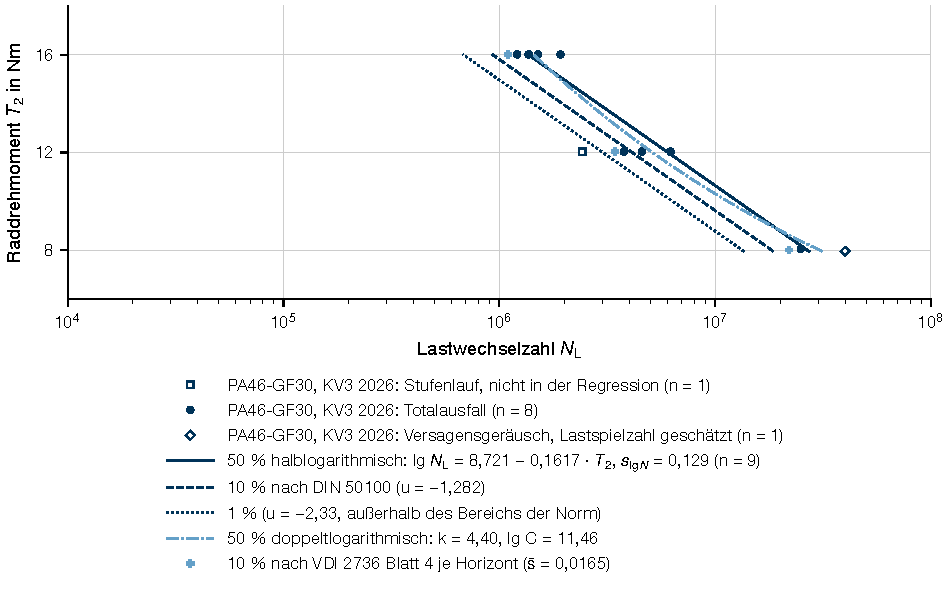
\includegraphics[width=\textwidth]{kap6/woehler_T2_pa46gf30_kv3_2026}
    \caption{Wöhlerlinie der Räder aus PA46-GF30 über dem Raddrehmoment: Punkte je Kriterium, halblogarithmische Gerade für $50$\,\% mit den parallelen Linien für $10$ und $1$\,\% Ausfallwahrscheinlichkeit nach DIN 50100, doppeltlogarithmische Gerade und die Werte für $10$\,\% nach VDI 2736 Blatt 4 je Horizont.}
    \label{fig:woehler_T2_pa46gf30}
\end{figure}

Die halblogarithmische Gerade nach \eqref{eq:halblog_gerade} lautet mit $T_{2}$ in Nm
\begin{equation}
\lg N_{\mathrm{L},50\%} = 8{,}721 - 0{,}1617 \, T_{2} ,
\label{eq:woehler_pa46_halblog}
\end{equation}
gültig zwischen $8$ und $16$\,Nm. Die gepoolte Standardabweichung von $\lg N_{\mathrm{L}}$ beträgt $0{,}125$ und nach der Korrektur für den Stichprobenumfang $0{,}129$; sie liegt über der Untergrenze von $0{,}10$. Die doppeltlogarithmische Gerade nach \eqref{eq:zeitfestigkeitsgerade} liefert den Neigungsexponenten $k = 4{,}40$ mit $\lg C = 11{,}46$ und eine korrigierte Standardabweichung von $0{,}100$. Beide Geraden fallen bei $12$\,Nm zusammen. An den Rändern des belegten Bereichs weichen sie um höchstens $0{,}06$ Dekaden voneinander ab. \tabref{tab:woehler_horizonte} stellt je Horizont die gemessenen Lastwechselzahlen den Werten der Geraden für $50$, $10$ und $1$\,\% nach DIN 50100 gegenüber, daneben die Schätzwerte nach VDI 2736 Blatt 4. Die Richtlinie mittelt die normierten Standardabweichungen der Horizonte zu $\bar{s} = 0{,}0165$; daraus folgen Faktoren von $0{,}70$ bis $0{,}74$ zwischen $10$ und $50$\,\%, die Norm liefert mit der gepoolten Standardabweichung $0{,}68$. Die Linie für $1$\,\% ist eine Extrapolation über den Bereich der Norm hinaus und wird nur zum Vergleich mit den Festigkeitswerten der Stahlräder geführt.

\begin{table}[htbp]
    \caption{Horizonte der Wöhlerversuche mit PA46-GF30: gemessene Lastwechselzahlen, Werte der halblogarithmischen Geraden für $50$, $10$ und $1$\,\% nach DIN 50100 sowie Schätzwerte nach VDI 2736 Blatt 4 mit der Standardabweichung $s_{i}$ des Horizonts; Lastwechsel in $10^{6}$.}
    \label{tab:woehler_horizonte}
    \centering
    \footnotesize
    \setlength{\tabcolsep}{4pt}
    \begin{tabular}{L{1.2cm}L{0.6cm}L{3.2cm}L{1.3cm}L{1.3cm}L{1.3cm}L{1.5cm}L{1.2cm}L{1.5cm}}
        $T_{2}$ in Nm & $n$ & gemessen & $N_{\mathrm{L},50\%}$ & $N_{\mathrm{L},10\%}$ & $N_{\mathrm{L},1\%}$ & $N_{i,50\%}$ VDI & $s_{i}$ & $N_{i,10\%}$ VDI \\
        \hline
        $8$ & $2$ & $24{,}96$ / $40{,}0$ geschätzt & $26{,}7$ & $18{,}2$ & $13{,}3$ & $31{,}6$ & $0{,}145$ & $22{,}0$ \\
        $12$ & $3$ & $3{,}78$ / $4{,}57$ / $6{,}21$ & $5{,}96$ & $4{,}07$ & $2{,}98$ & $4{,}75$ & $0{,}109$ & $3{,}44$ \\
        $16$ & $4$ & $1{,}21$ / $1{,}37$ / $1{,}51$ / $1{,}92$ & $1{,}36$ & $0{,}93$ & $0{,}68$ & $1{,}48$ & $0{,}085$ & $1{,}10$ \\
    \end{tabular}
\end{table}

Die Streuung auf dem Horizont $8$\,Nm trägt die geschätzte Lastwechselzahl des Laufs kst-E\_75 und den Lauf kst-E\_69 mit dem erhöhten Moment in der ersten Million Lastwechsel; beide Punkte gehen ohne Gewichtung ein. Mit zwei Rädern auf dieser Stufe stützt sich die Lage der Geraden bei $8$\,Nm auf die Neigung aus den Stufen $12$ und $16$\,Nm. Die Linie wird nicht über $8$\,Nm hinaus verlängert, und ein Abknicken in eine Langzeitfestigkeit ist mit den Daten nicht belegbar.

Zur Prüfung der Verteilung wurden die Lastwechselzahlen auf den Wert der halblogarithmischen Geraden ihres Horizonts bezogen und nach der Größe geordnet. Mit den Ausfallwahrscheinlichkeiten nach Rossow und nach $j/(n+1)$ stehen sie im Gauß-Netz in \figref{fig:netz_gauss_pa46gf30} und im Weibull-Netz in \figref{fig:netz_weibull_pa46gf30}. \tabref{tab:woehler_netze} nennt die Geraden der Netze. Beide Verteilungen beschreiben die neun Punkte mit Bestimmtheitsmaßen zwischen $0{,}962$ und $0{,}971$; der Unterschied trägt bei diesem Stichprobenumfang keine Entscheidung. Die logarithmische Normalverteilung wird beibehalten, wie DIN 50100 sie vorsieht, und die Streuung aus dem Gauß-Netz mit $0{,}125$ stimmt mit der gepoolten Standardabweichung der Regression überein. Der Formparameter der Weibull-Verteilung liegt mit $3{,}7$ bis $4{,}3$ nahe dem Wert $3{,}46$, den Illenberger für die Grübchentragfähigkeit von PEEK-Rädern findet, und nahe dem Wert $3{,}6$, bei dem die Weibull-Verteilung der Normalverteilung entspricht \cite[S.~96 bis 97]{Ill22}. Die Faktoren von $50$ auf $10$\,\% betragen $0{,}66$ bis $0{,}69$ nach dem Gauß-Netz und $0{,}60$ bis $0{,}64$ nach dem Weibull-Netz, gegenüber $0{,}58$ bei Illenberger und $0{,}70$ bis $0{,}74$ nach VDI 2736 Blatt 4.

\begin{figure}[htbp]
    \centering
    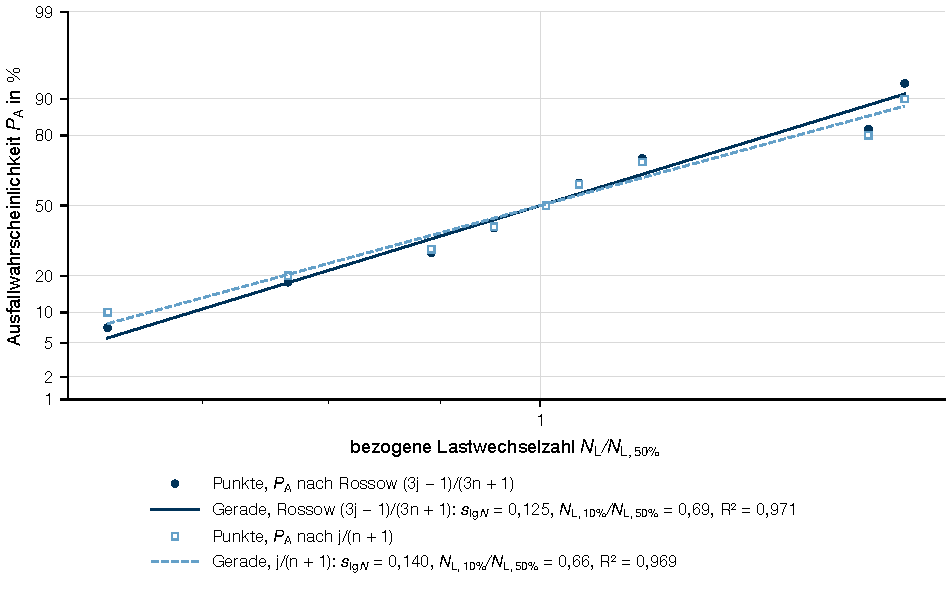
\includegraphics[width=\textwidth]{kap6/netz_gauss_pa46gf30_kv3_2026}
    \caption{Gauß-Netz der auf die Gerade für $50$\,\% bezogenen Lastwechselzahlen der neun Wöhlerversuche mit PA46-GF30, Ausfallwahrscheinlichkeit nach Rossow und nach $j/(n+1)$.}
    \label{fig:netz_gauss_pa46gf30}
\end{figure}

\begin{figure}[htbp]
    \centering
    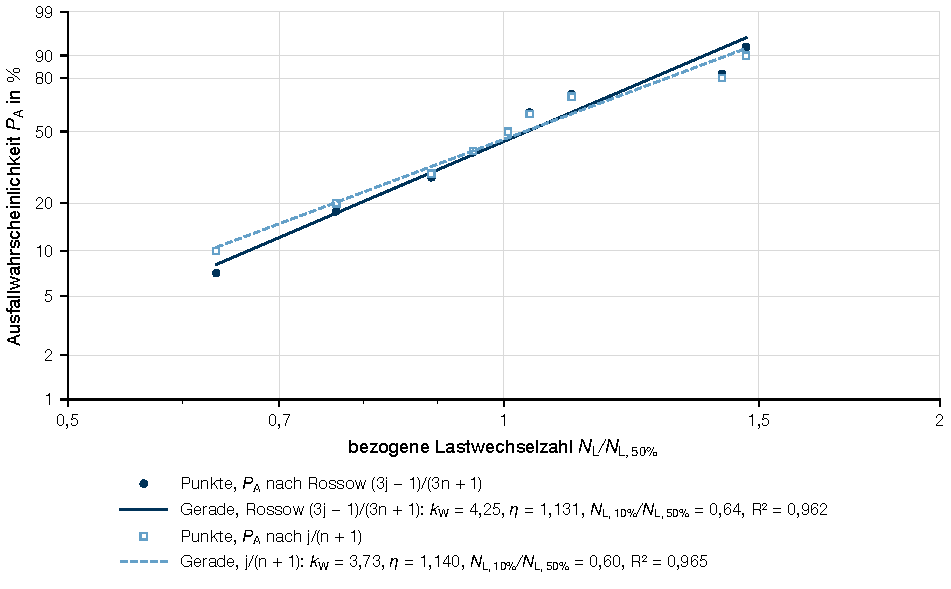
\includegraphics[width=\textwidth]{kap6/netz_weibull_pa46gf30_kv3_2026}
    \caption{Weibull-Netz der auf die Gerade für $50$\,\% bezogenen Lastwechselzahlen der neun Wöhlerversuche mit PA46-GF30, Ausfallwahrscheinlichkeit nach Rossow und nach $j/(n+1)$.}
    \label{fig:netz_weibull_pa46gf30}
\end{figure}

\begin{table}[htbp]
    \caption{Geraden in den Wahrscheinlichkeitsnetzen der bezogenen Lastwechselzahlen: Standardabweichung $s_{\lg N}$ des Gauß-Netzes, Formparameter $k_{\mathrm{W}}$ und charakteristische Lebensdauer $\eta$ des Weibull-Netzes, Faktoren von $50$ auf $10$ und $1$\,\% sowie Bestimmtheitsmaß $R^{2}$.}
    \label{tab:woehler_netze}
    \centering
    \footnotesize
    \begin{tabular}{L{1.6cm}L{2.6cm}L{2.4cm}L{2.0cm}L{1.6cm}L{1.6cm}L{1.4cm}}
        Netz & $P_{\mathrm{A}}$ nach & $s_{\lg N}$ bzw. $k_{\mathrm{W}}$ & $10^{\mu}$ bzw. $\eta$ & $N_{10\%}/N_{50\%}$ & $N_{1\%}/N_{50\%}$ & $R^{2}$ \\
        \hline
        Gauß & Rossow & $0{,}125$ & $1{,}000$ & $0{,}69$ & $0{,}51$ & $0{,}971$ \\
        Gauß & $j/(n+1)$ & $0{,}140$ & $1{,}000$ & $0{,}66$ & $0{,}47$ & $0{,}969$ \\
        Weibull & Rossow & $4{,}25$ & $1{,}131$ & $0{,}64$ & $0{,}37$ & $0{,}962$ \\
        Weibull & $j/(n+1)$ & $3{,}73$ & $1{,}140$ & $0{,}60$ & $0{,}32$ & $0{,}965$ \\
    \end{tabular}
\end{table}

Für die Versagensdefinition des Nachweises nach Stommel et al. liefern die Sichtkontrollen die Anrissfenster aus \tabref{tab:versuchsprogramm_pa46}. Auf der Stufe $8$\,Nm lagen die ersten sichtbaren Anrisse beim Rad 97345 zwischen $13$ und $31$\,\% der Lastwechsel bis zum Ende, beim Rad 97364 zwischen $9$ und $17$\,\%. Mehr als zwei Drittel der Laufzeit vergingen auf dieser Stufe mit sichtbaren Rissen. Auf den Stufen $12$ und $16$\,Nm ist in der ersten Million Lastwechsel keine Kontrolle ohne Befund dokumentiert. Die erste Kontrolle mit Befund nennt dort nur eine obere Schranke, die zwischen $55$ und $93$\,\% der Laufzeit liegt. Der Vergleich mit dem Nachweis folgt in \secref{sec:genauigkeit}. \Note{PH: Wöhlerbilder über der Zahnfußspannung $\sigma_{\mathrm{F}}$ je Verfahren und über $\sigma_{1}$ des FE-Modells, sobald die Spannungen je Drehmoment aus \secref{sec:verfahrensvergleich} vorliegen; dort auch die Werte für PA66 nach VDI 2736 Blatt 2.}

% Herkunft:
% Absatz 1 bis 3 (Geraden, Horizonte): 80_output/messungen/woehler/woehler.md (measurements.py woehler, L2):
%   halblogarithmisch a_c 8,7205, b_c 0,16166, s 0,1247, korrigiert 0,1293; doppeltlogarithmisch lg C 11,4617,
%   k 4,404, s 0,0965, korrigiert 0,1001; Horizonte 8 Nm 24 956 000 / 40 000 000, N50 2,671e7, N10 1,823e7, N1
%   1,334e7, VDI 3,159e7, s_i 0,1449, N10 2,195e7; 12 Nm 3 776 250 / 4 570 000 / 6 213 262, 5,964e6, 4,071e6,
%   2,980e6, 4,751e6, 0,1091, 3,435e6; 16 Nm 1 210 000 / 1 366 000 / 1 512 000 / 1 920 000, 1,357e6, 9,266e5,
%   6,782e5, 1,480e6, 0,0851, 1,097e6; s quer 0,01648. Faktoren VDI: 10^(−1,28 · 0,01648 · L_i,50) = 0,695/0,723/
%   0,741; DIN 10^(−1,282 · 0,1293) = 0,683. Abstand der Geraden: bei 8 Nm lg 2,671e7 = 7,427 gegen
%   11,4617 − 4,404 · lg 8,00 = 7,484 (0,057 Dekaden); bei 16 Nm 6,133 gegen 6,158 (0,025).
% Absatz 4 (8 Nm): test_runs_user.yaml (69, 75); DIN 50100 S. 16 und 59 über 2.6.
% Absatz 5 bis 7 (Netze): woehler.md Tabelle Netze (Gauß rossow 0,1249/1,0000/0,692/0,512/0,9707; rank
%   0,1400/0,661/0,472/0,9690; Weibull rossow 4,2539/1,1308/0,642/0,370/0,9623; rank 3,7342/1,1403/0,604/0,322/
%   0,9648); Illenberger2022.txt Druckseite 96 (k = 3,46, f10 0,58), 97 (k = 3,602 ≈ Normalverteilung).
% Absatz 8 (Anrissfenster): anrissfenster.md; Anteile: 69 3,223/24,956 = 0,13 und 7,658/24,956 = 0,31; 75
%   3,653/40 = 0,09 und 6,610/40 = 0,17; 74 2,53/4,57 = 0,55; 70 1,404/1,512 = 0,93; 71 0,962/1,210 = 0,79; 72
%   0,945/1,366 = 0,69; 73 1,719/1,920 = 0,90; ADR-118 Amendment 2026-10-18 Abend Punkt 1 (dreistufiger
%   Vergleich in 7.1).
% Bildwunsch: kap6/woehler_T2_pa46gf30_kv3_2026, kap6/netz_gauss_pa46gf30_kv3_2026, kap6/netz_weibull_pa46gf30_kv3_2026
%   (bilder.yaml).
% Bibwunsch: Ill22 vorhanden.
% Nomenklatur: k_W, -, Formparameter der Weibull-Verteilung (Illenberger S. 96: k); eta, -, charakteristische
%   Lebensdauer der Weibull-Verteilung, bezogen (63,2 %); mu, -, Lage der bezogenen Lastwechselzahl im Gauß-Netz
%   (lg); R^2, -, Bestimmtheitsmaß; N_L,50 % usw. über N_L; s_lgN, P_A, j, n, u, s_i, s quer, C, k aus 2.6.
% Offen: Abszissen sigma_F und sigma_1 (nach C7 und L6b); Verweis sec:genauigkeit (7.1, noch nicht entworfen).
